\item Se va a construir una canaleta para agua de lluvia con lámina metálica de 30 cm de ancho, doblando la tercera parte de la hoja en cada uno de sus lados un ángulo $\theta$. Determine el valor de tal ángulo $\theta$ que permita que el canal conduzca la máxima cantidad de agua.
\begin{center}
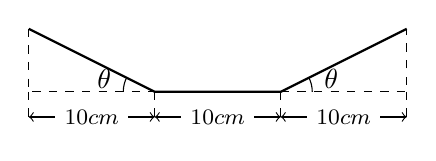
\begin{tikzpicture}[scale=0.8]
    \draw[thick] (-2,1) -- (0,0) -- (2,0) -- (4,1);
    \draw[dashed] (-2,1) -- (-2,0) -- (0,0);
    \draw[dashed] (2,0) -- (4,0) -- (4,1);
    \draw (-0.5, 0) arc (180:153:0.5);
    \node at (-0.8, 0.2) {$\theta$};
    \draw (2.5, 0) arc (0:27:0.5);
    \node at (2.8, 0.2) {$\theta$};
    \draw[<->] (-2, -0.4) -- (0, -0.4) node[midway, fill=white] {\footnotesize $10 \text{ cm}$};
    \draw[<->] (0, -0.4) -- (2, -0.4) node[midway, fill=white] {\footnotesize $10 \text{ cm}$};
    \draw[<->] (2, -0.4) -- (4, -0.4) node[midway, fill=white] {\footnotesize $10 \text{ cm}$};
    \draw[dashed] (-2,0) -- (-2,-0.5);
    \draw[dashed] (0,0) -- (0,-0.5);
    \draw[dashed] (2,0) -- (2,-0.5);
    \draw[dashed] (4,0) -- (4,-0.5);
\end{tikzpicture}
\end{center}
